\chapter{Anhang} \label{chpt:Anhang_Main}


Hier sind noch \LaTeX-Beispiele für die Verwendung: 

...
\newline
\newline
Tabelle erzeugen: 
\begin{table}[htbp]
	\centering
	\caption{Beispieltabelle}
	\begin{tabularx}{\textwidth}{|X|X|X|X|}
		\hline
		Spalte 1 & Spalte 2 & Spalte 3 & Spalte 4 \\
		\hline
		Inhalt 1 & Inhalt 2 & Inhalt 3 & Inhalt 4 \\
		\hline
		Inhalt 5 & Inhalt 6 & Inhalt 7 & Inhalt 8 \\
		\hline
	\end{tabularx}
\end{table}

...
\newline
\newline
Quellen verlinken: 
% Quellenverlinkung
Test \cite{Bar-Shalom}.
Test \cite{Goldhammer}.
Test \cite{WHO-2004}.

...
\newline
\newline
Kapitel verlinken: 
% Kapitelverlinkung
Wie in Abschnitt \ref{chpt:Ergebnisse_Main} beschrieben wird ...

...
\newline
\newline
% Einfügen einer Grafik/Bildes etc.
\begin{figure}[ht]
	\centering
	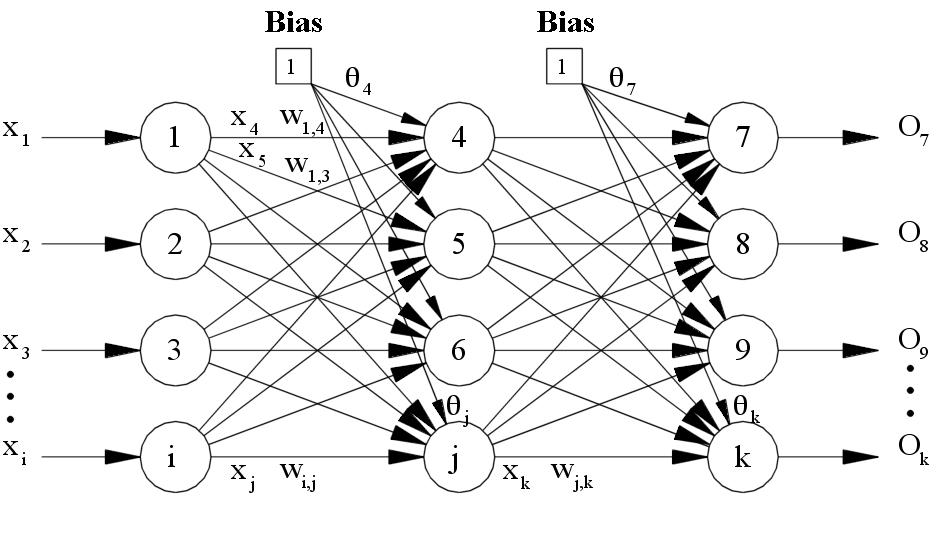
\includegraphics[scale=0.40]{Bilder/Neural_Network.jpg}
	\caption{Beispielbild}
	\label{fig: Neural_Network_Fig}
\end{figure}



